%http://www.etaps.org/index.php/2014/cc
%to be submtitted to https://www.easychair.org/account/signin.cgi?timeout=1;conf=cc2014
% abstract: 4th october 2013
% paper: 11th october 2013
%
%Submissions should consist of two parts:
%
%    The first part, at most 4 pages, should describe the tool presented. Please include the URL of the tool (if available) and provide information that illustrates the maturity and robustness of the tool (this part will be included in the proceedings).
%        The second part, at most 6 pages, should explain how the demonstration will be carried out and what it will show, including screen dumps and examples. (This part will be not be included in the proceedings, but will be evaluated.)
%
\documentclass{llncs}

\usepackage{listings}
\usepackage{url}
\usepackage{acronym}
\usepackage{todo}
\usepackage{paralist}
\usepackage[english]{babel}

\usepackage{tikz}
\usetikzlibrary{backgrounds}
\usetikzlibrary{calc}
\usetikzlibrary{positioning}
\usetikzlibrary{shadows}
\usetikzlibrary{arrows}
\usetikzlibrary{shapes}
\usetikzlibrary{fit}

\bibliographystyle{splncs}
\lstset{language=python,morekeywords={cimport, cdef, with},
basicstyle=\ttfamily, keywordstyle=\bf, stringstyle=\color{gray},
captionpos=b}

\acrodef{AST}{Abstract Syntax Tree}
\acrodef{API}{Application Programming Interface}
\acrodef{CLI}{Command Line Interface}
\acrodef{IR}{Internal Representation}
\acrodef{JIT}{Just-In-Time}
\acrodef{AOT}{Ahead-Of-Time}
\acrodef{OO}{Object Oriented}
\acrodef{OSS}{Open Source Software}

\title{Pythran: Turning Python Modules into Optimized C++ Meta-Programs}

\author{Serge Guelton\inst{1,2} \and Pierrick Brunet\inst{2}}

\institute{\'Ecole Normale Sup\'erieure, D\'epartement d'Informatique, Paris, France
\and
T\'el\'ecom Bretagne, Plouzan\'e, France
}
\begin{document}


\maketitle

\begin{abstract}

    Pythran is a compiler tool that turns source files written in a subset of
    the Python language into C++11 meta-programs. It also extract from the
    original source files type annotations used to instantiate the meta-programs
    into a Python native module that runs typically faster than its interpreted
    counterpart.

    This paper presents the optimization techniques the Pythran compiler applies
    to Python code: unboxing, deforestation, inter procedural constant folding,
    explicit and implicit parallelization and implicit vectorization.

\end{abstract}

\section{Introduction}

Python is a renowned programming language that supports multiple paradigms. It
is highly dynamic (e.g.\ typing and name resolution are dynamic) at the expense
of slower execution than equivalent programs written in static languages.

Several tools exist to counterbalance the execution time limitations. They can
be classified depending on
% PB : Inline enumeration looks strange for me but may be it is the english way to do
\begin{inparaenum}[1)]
\item the restriction they impose on their input and
\item the compilation approach.
\end{inparaenum}
PyPy\cite{pypy2009} targets the whole Python
language using a tracing \ac{JIT} approach, Nuitka\cite{nuitka2012} sets the same
goal but using translation to C++ and \ac{AOT} compilation.
Shed~Skin\cite{shedskin2006} translates to C++ but only targets an implicitly statically
typed subset of Python and several modules from the standard library. In the
field of numerical computations, Parakeet\cite{parakeet2012} and
Numba\cite{numba2013} are \ac{JIT} compilers based on LLVM that
only supports the Python subset required to run numpy-centric programs.

Pythran\cite{pythran2013} is an \ac{AOT} compiler that focuses on the
optimization of the functional and procedural paradigms offered by Python,
leaving aside dynamicity and most \ac{OO} features to focus on scientific python modules.  Indeed, the Python
language and its standard library offers comprehensive services to the
programmers, but the language proves to be useful even with a limited subset of
features:
\begin{inparaenum}[1)]
\item classical data types (\texttt{bool}eans, \texttt{int}egers,
\texttt{long} integers, \texttt{float}ing point numbers, \texttt{str}ings)~;
\item standard containers (\texttt{list}s, \texttt{set}s, \texttt{tuple}s,
\texttt{dict}ionaries) ;
\item a few features or function inherited from
functional programming such as \texttt{list}/\texttt{set}/\texttt{dict}
comprehension and \texttt{reduce}, \texttt{map}, \texttt{filter} operators and
\item the \texttt{numpy} module that
provides a multi-dimensional array structure targeted at scientific computing. 
% "at scientific computing" looks strange for me but it may be my bad english...
\end{inparaenum}

The paper is organized as follows: Section~\ref{sec:architecture} presents the
architecture of the Pythran compiler, Section~\ref{sec:functionnal-optim}
details some high-level optimizations related to the functional aspects of
Python, while Section~\ref{sec:numeric-optim} focuses on optimizations for
numerical computations.

\section{Architecture of the Pythran Compiler}
\label{sec:architecture}

% mature?
% yes, mature! 1500+ validation test looks mature enough to me ;-)
Pythran is an \ac{OSS} available through its source code
repository (see \url{https://githib.com/serge-sans-paille/pythran}), the
Python Package Index (see \url{https://pypi.python.org/pypi/pythran}) and
a Debian repository (see \url{http://ridee.enstb.org/debian}). It can be
used as a source-to-source compiler infrastructure for a subset of the Python
language, a C++11 meta-programs generator or a native module generators. Each
of this target corresponds to a layer in the tool architecture described in
Figure~\ref{fig:archi}.

The \ac{IR} used by Pythran is a strict subset of Python's \ac{AST}, simplified
to ease the optimization process. Using a high-level \ac{IR} is well suited for
high-level transformations, and provides source-to-source facilities for free.
As the primary backend of Pythran is C++11, a high-level language, there is no
need of low-level optimizations that are performed by the backend compiler.

% It looks like pythran generate a *.py file as an output. What did you mean with
% this arrow?
% SG: Pythran can generate a.py file if using the Python backend
\begin{figure}[ht]
    \centering
    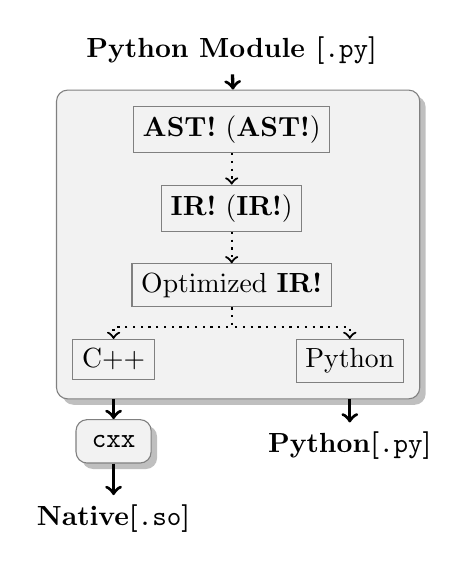
\begin{tikzpicture}[
            file/.style={align=center, node distance=0.4cm},
            state/.style={draw=black!50,fill=black!5,rectangle, align=center, node distance=0.4cm},
            box/.style={draw=black!50,fill=black!5,rectangle, rounded corners, drop shadow, align=center,
            node distance=0.4cm, inner sep=.2cm},
            mbox/.style={draw=black!50,fill=black!5,rectangle, rounded corners, drop shadow, align=center,
            node distance=0.4cm, inner sep=.2cm},
        ]
        \node[file] (python)                      {\textbf{Python Module [\texttt{.py}]}};
        \node[state] (ast)       [below=of python]       {\ac{AST}};
        \node[state] (ir)        [below=of ast]          {\ac{IR}};
        \node[state] (ir2)       [below=of ir]           {Optimized \ac{IR}};
        \node[state] (be0)       [xshift=1.5cm, below=of ir2]          {Python};
        \node[state] (be1)       [xshift=-1.5cm,below=of ir2]          {C++};
        \begin{pgfonlayer}{background} 
            \node[box]  (pythran)   [fit=(ast) (ir) (be0) (be1)]  {};
        \end{pgfonlayer}
        \node[mbox] (cxx)        [yshift=-.1cm, below=of be1]          {\texttt{cxx}};
        \node[file] (so)        [below=of cxx]          {\textbf{Native[\texttt{.so}]}};
        \node[file] (py)        [yshift=-.1cm, below=of be0]          {\textbf{Python[\texttt{.py}]}};


        \draw[very thick, ->] (python) -- (pythran);
        \draw[very thick, ->] (pythran.south -| cxx.north) -- (cxx.north);
        \draw[very thick, ->] (cxx) -- (so);
        \draw[very thick, ->] (pythran.south -| py.north) -- (py.north);

        \draw[thick, dotted, ->] (ast) -- (ir);
        \draw[thick, dotted, ->] (ir) -- (ir2);
        \draw[thick, dotted, ->] (ir2.south) -- ($(ir2.south) - (0, .25)$) -| (be0.north);
        \draw[thick, dotted, ->] (ir2.south) -- ($(ir2.south) - (0, .25)$) -| (be1.north);

    \end{tikzpicture}

    \caption{Architecture of the Pythran compiler.}
    \label{fig:archi}
\end{figure}


The compilation process used by Pythran follows several steps:
% In previous enumeration, all items are in a same sentence, here we have
% a sentence for each item.
\begin{inparaenum}[1)]
\item\label{en:ast} Turn Python code into an \ac{AST} using the \texttt{ast}
    module.
\item Refine Python \ac{AST} into Pythran \ac{IR}. For instance this makes
    \emph{destructuring} or \emph{list comprehension} explicit and removes the
    corresponding constructs from the \ac{AST}. \emph{Partial functions} or
    %what is partial function in python? Is it sub-function
    % (function declared in another function)?
    \emph{lambda functions} are also converted to top-level functions after
    closure computations at this step.
\item Perform several optimizations on the \ac{IR}, using the optimization
    sequence provided by the user.
    %after user optimisation, it applies pythran default optimisation, isn't it?
\item Type the \ac{IR} using \emph{parametric types}.
\item Dump the \ac{IR} into Python code or templated C++ code.
\item Optionally use type annotations gathered during Step~\ref{en:ast} to
    instantiate the C++ meta-functions and compile them to native code.
\end{inparaenum}

The compiler can be used from the \ac{CLI} as a regular Python-to-native-code
compiler that takes a \texttt{.py} module and turns it into a \texttt{.so}
native module. It can also be used as a compiler infrastructure, in which case
the developer interacts with the various passes and analyse through the
\texttt{PassManager} class.

\section{Procedural and Functional Python Optimizations}
\label{sec:functionnal-optim}

% PB : --- are ugly for me :-) but it is only cosmetic
Python compilers generally use \emph{unboxing}---the process of removing the
object layer Python adds around any value---as the primary way to obtain
C-like performances. This is achieved either through the discovery of variable
types at runtime or through static typing. Pythran, in a similar manner to
Sched Skin, relies on static type inference, with the slight difference that it
performs function-level parametric typing and relies on C++ template
instantiantion to verify the code is correctly type. In the end, valid Pythran
programs are implicitly statically typed and all variables are unboxed.
% PB : I don't understand where pythran unbox values.

Additionally, Pythran performs several optimizations inherited from functional
programing to its \ac{IR}. It uses a variant of
\emph{deforestation}~\cite{Wadler1988} to avoid usage of intermediate storage
when combining some intrinsics. Practically, this relies on aliasing analysis
to detect calls to the \texttt{map} (resp.\ \texttt{range}, \texttt{zip} or
\texttt{filter}) functions and lazyness analysis to turn them into calls to the
% and pure function detection?
\texttt{imap} function from the \texttt{itertools} module (resp.\
\texttt{xrange}, \texttt{izip} or \texttt{ifilter}). The transformation engine
is aware of the semantics of several Python builtins, so that a call like
\texttt{sum(map(sqrt, map(abs, l))} is turned into the equivalent---but more
% PB : explains why it is more efficient?
memory-efficient---\texttt{sum(imap(sqrt, imap(abs, l))}. During its \ac{AST}
to \ac{IR} conversion, Pythran turns some list comprehension constructs into
\texttt{map} calls, so list comprehension also benefit from the optimization:
\texttt{sum([x*y for x,y in zip(l0, l1)]} is turned into \texttt{sum(imap(foo,
izip(l0, l1)))}, where \texttt{foo} is an helper function generated on the fly.

Using the introspection ability of Python, Pythran also performs
inter-procedural constant folding. The optimization relies on an analysis that
flags some functions as ``pure'' when they neither update their arguments not
have global side effects (which include I/O and random generator state). When a
pure function is called without arguments or with literal arguments, it can be
replaced by its compile-time evaluation. Technically, as Pythran's\ac{IR} is a
subset of Python's \ac{AST}, a simple call to the \texttt{eval} builtin yields
the result to substitute.

\section{Numeric Python Optimizations}
\label{sec:numeric-optim}

Thanks to the \texttt{scipy} and \texttt{numpy} packages, Python is also used
for fast prototyping of numerical applications. Pythran
implements part of the \acs{API} of the \texttt{numpy} package, with a focus on
the multi-dimensional array point-to-point expressions. Given two arrays of
similar shape \texttt{a} and \texttt{b}, it turns the expression
\texttt{cos(a)*sin(2*b)} into a single parallelized and vectorized loop, taking
advantage of multiple cores and vector instruction units if available. This is
done at the C++ level using algorithmic patterns parallelized with OpenMP,
vectorized through calls to \texttt{Boost.simd}~\cite{boostsimd2012} and
combined with \emph{expression template}s.

To parallelize explicit loops, Pythran makes it possible to use the OpenMP
syntax at the Python level, as described in~\cite{pythranOMP2013}. Following
the original OpenMP philosophy, OpenMP annotations are added to the sequential
program to give it an additional parallel semantic, either loop-based or
task-based. Annotations can be discarded by the compiler to keep the original
sequential semantics.

\section{Conclusion}

The Pythran compiler offers a robust (the validation suite holds more than 1500
test cases) tool to translate procedural Python modules into natives ones. It
can also be used as a compiler infrastructure that offers high-level analysis
like points-to analysis, global effects analysis etc.

It is of interest for Python user that needs to prototype algorithms and make
them run at C-speed without the burden of writing low-level code. It can also
be used as a clean compiler infrastructure, using Python \ac{AST} as a
common \ac{IR}.

\bibliography{biblio}

\end{document}
